\subsection{\glspl{MSR}}

\begin{frame}
\frametitle{MSR (Molten Salt Reactor) types}
\begin{textblock*}{12cm}(0.4cm,2.1cm) % {block width} (coords)
	\begin{overlayarea}{\linewidth}{20\baselineskip}
		\begin{block}{Stationary Fuel}<1-4>
			\begin{enumerate}
				\item \textbf{Solid}
				\begin{itemize}
					\item Graphite block with TRISO fuel, clean salt works as 
					coolant (Fluoride-Salt-Cooled High-Temperature Reactor 
					(FHR))
					\item Plate Fuel: hexagonal fuel assembly is similar in 
					shape 
					to a typical sodium-cooled reactor
					\item Fuel Inside Radial Moderator (FIRM)
				\end{itemize}
			\end{enumerate}
		\end{block}
		
		\begin{block}{Mobile Fuel}<2-4>
			\begin{enumerate}
				\item \textbf{Solid}
				\begin{itemize}
					\item<2-> Mobile solid fuel elements (pebbles) cooled by 
					clean salt (PB-FHR by Kairos Power)
				\end{itemize}
				\item<3-> \textbf{Liquid}
				\begin{itemize}
					\item<3-> Without on-site fuel reprocessing facility 
					(TerraPower \glsfirst{MCFR})
					\item<4-> \textbf{With on-site fuel reprocessing} 
					(\glsfirst{TAP} MSR, \glsfirst{MSBR})
				\end{itemize}
			\end{enumerate}
		\end{block}
	\end{overlayarea}
\end{textblock*}
\end{frame}

\begin{frame} % Add another slide with red rectangular around reprocessing 
%system
\frametitle{Circulating-fuel reactor with on-site reprocessing system}
% Weinberg 1945, U sulfate in water, 140kW
\vspace{-2mm}
\begin{figure}[t]
		\begin{overprint}
			\onslide<1>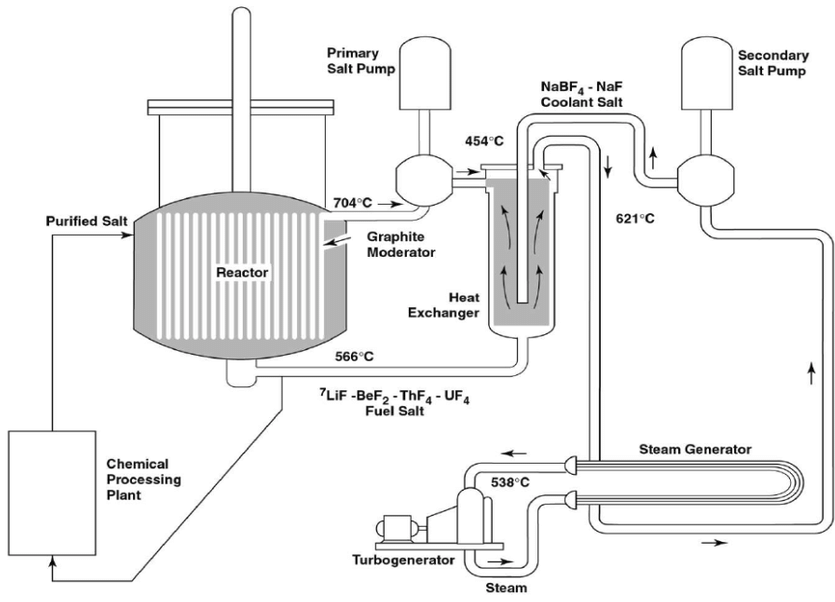
\includegraphics[height=0.6\textwidth]{./images/msbr_scheme.png}
			\onslide<2>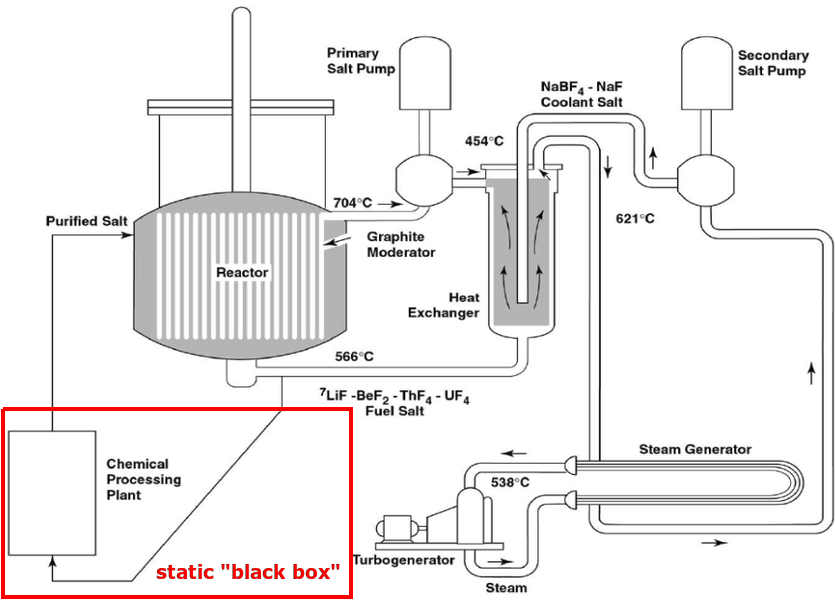
\includegraphics[height=0.6\textwidth]{./images/msbr_scheme_box.png}
		\end{overprint}
	\caption{The MSBR is an example of reactor design with 
	\textbf{liquid, mobile, circulating} fluoride salt fuel 
	(reproduced from Rosenthal \emph{et al.} 
	\cite{rosenthal_molten-salt_1970}).}
\end{figure}   

\end{frame}

\begin{frame}
\frametitle{Why Molten Salt Reactors with circulating fuel?}
\begin{block}{Liquid-fueled \gls{MSR} designs have following \textbf{potential} advantages:}
	\begin{enumerate}
		\itemsep1em
		\item High coolant temperature (600-750$^{\circ}$C) 
		$\Rightarrow$ potentially high thermal efficiency, process 
		heat for chemical industry or hydrogen production
		\item Fuel diversity ($^{235}$U, $^{233}$U, Thorium, U/Pu)
		\item Strong negative fuel temperature feedback 
		\item Passive safety $\Rightarrow$ fuel drains into tanks 
		in emergency
		\item High fuel utilization $\Rightarrow$ reduced spent fuel 
		generation
		\item<2> \textbf{On-line (continuous) fuel reprocessing and refueling}
	\end{enumerate}
\end{block}

\end{frame}


\subsection{Background}

\begin{frame}
\frametitle{On-line fuel processing and on-line refueling pros and 
cons}
\begin{block}{Advantages}
	\begin{enumerate}
		\item Neutron economy
		\item Fuel utilization
		\item Refueling without outages
		\item Reduced excess reactivity
	\end{enumerate}
\end{block}

\begin{block}{Disadvantages}
	\begin{enumerate}
		\item Chemical separation is challenging
		\item Fuel salt balance in the primary loop complicates operation
		\item \textbf{Existing burnup calculation software cannot model it}
	\end{enumerate}
\end{block}

\end{frame}


\begin{frame}
\frametitle{Fuel salt burnup and reprocessing}
		\vspace{-5mm}
	\begin{figure}[t]
		\hspace*{-0.2in}
			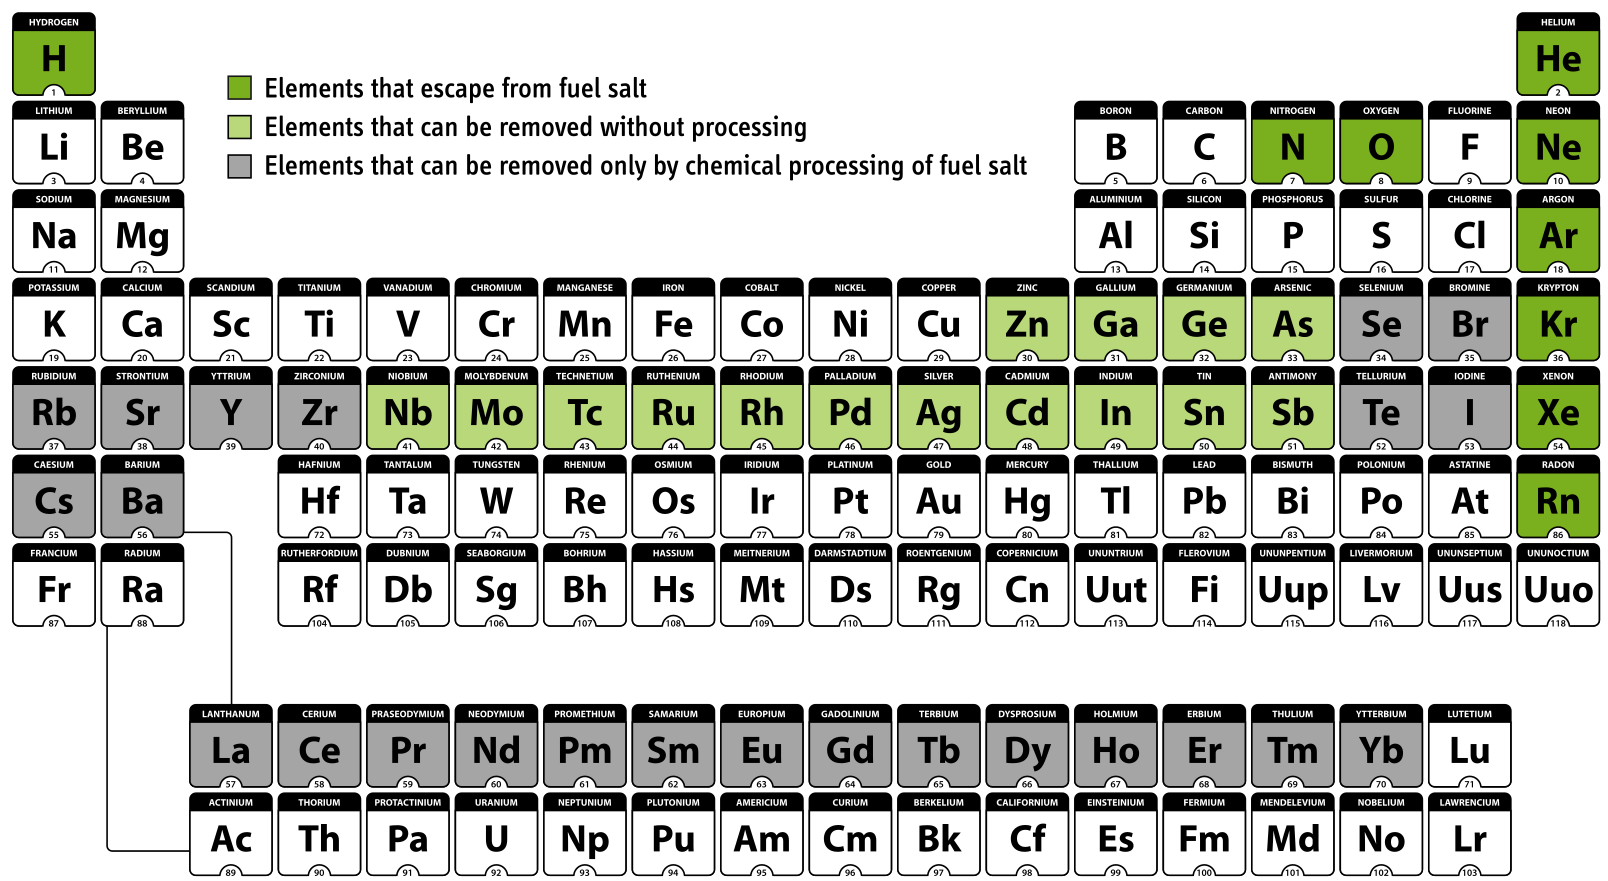
\includegraphics[height=0.6\textwidth]{./images/periodic_map.png}
		\vspace{-0.15in}
		\caption{Processing options for MSR fuels (figure reproduced from Ahmed \emph{et al.}  \cite{ahmad_neutronics_2015}).}
	\end{figure}               
\end{frame}


\begin{frame}
\frametitle{On-line fuel salt reprocessing system functions}
\begin{block}{Removing poisonous fission products}
	\begin{itemize}
		\item Noble gas (e.g., centrifugal gas separator)
		\item Noble metal (e.g., large filter with nickel fibers)
       \item Rare earth (separation based on different chemical potentials)
		%\item Ideally, remove 100\% of target element but realistically, 
		%30-90\%
		\item Some valuable rare metals (Rh,Pd) may be recovered %%Rh - $5000, 
%%%Pd - $1500, Pl - $900, Ir - $1480
	\end{itemize}
\end{block}

\begin{block}{Injecting fresh fuel}
	\begin{itemize}
		\item Fissile material ($^{233}$U, $^{235}$U, $^{239}$Pu)
		\item Fertile material ($^{232}$Th, $^{238}$U)
		\item Maintain fuel salt inventory in the primary loop
		\item Maintain reactor criticality (ideally, $k_{eff}=1.0$)
	\end{itemize}
\end{block}

\end{frame}

\begin{frame}
\frametitle{Continuous vs batch-wise fuel processing  and refueling (1/3)}
\vspace{-8mm}
\begin{block}{Classic Bateman equation}
	%Core material is circulated to or from the core at specific intervals:
	\begin{align}
	\frac{dN_i}{dt} &= \sum_{m=1}^{M}l_{im}\lambda_mN_m + 
	\phi\sum_{m=1}^{M}f_{im}\sigma_mN_m - (\lambda_i + \phi\sigma_i)N_i + 
	F_i\Big|\quad{i\in [1,M]} \nonumber\\
	N_i &= \mbox{atom density of nuclide i} \nonumber \\
	M &= \mbox{number of nuclides} \nonumber \\
	l_{im} &= \mbox{fraction of decays of nuclide m that result in formation 
	of 
		nuclide i}\nonumber \\
	\lambda_i &= \mbox{radioactive decay constant of nuclide i} \nonumber \\
	\phi &= \mbox{neutron flux, averaged over position and energy} \nonumber \\
	f_{im} &= \mbox{fraction of neutron absorption by nuclide m leading to the 
		formation of nuclide i} \nonumber \\
	\sigma_m &= \mbox{average neutron absorption cross section of nuclide m} 
	\nonumber \\
	F_i &= \mbox{production rate of nuclide i directly from fission}\nonumber
	\end{align}
\end{block}
\end{frame}

\begin{frame}
\frametitle{Continuous vs batch-wise fuel processing  and refueling (2/3)}
\vspace{-1.3mm}
\begin{block}{Bateman equation with continuous removals and feed}
	\begin{align}
	\frac{dN_i}{dt} &= \sum_{m=1}^{M}l_{im}\lambda_mN_m + 
	\phi\sum_{m=1}^{M}f_{im}\sigma_mN_m - (\lambda_i + \phi\sigma_i + 
	\textcolor{red}{r_i - 
		f_i})N_i + F_i\Big|\quad{i\in [1,M]} \nonumber \\
	N_i &= \mbox{atom density of nuclide i} \nonumber \\
	M &= \mbox{number of nuclides} \nonumber \\
	l_{im} &= \mbox{fraction of decays of nuclide m that result in formation 
	of 
		nuclide i}\nonumber \\
	\lambda_i &= \mbox{radioactive decay constant of nuclide i} \nonumber \\
	\phi &= \mbox{neutron flux, averaged over position and energy} \nonumber \\
	f_{im} &= \mbox{fraction of neutron absorption by nuclide m leading to the 
		formation of nuclide i} \nonumber \\
	\sigma_m &= \mbox{average neutron absorption cross section of nuclide m} 
	\nonumber \\
	\textcolor{red}{r_i} & \mkern4mu \textcolor{red}{=} \mbox{\space 
	\textcolor{red}{continuous removal rate of nuclide i from the system}} 
	\nonumber \\
	\textcolor{red}{f_i} & \mkern4mu  \textcolor{red}{=} \mbox{\space 
	\textcolor{red}{continuous feed rate of nuclide i}} \nonumber \\
	F_i &= \mbox{production rate of nuclide i directly from fission}\nonumber
	\end{align}
\end{block}
\end{frame}


\begin{frame}
\frametitle{Continuous vs batch-wise fuel processing and refueling (3/3)}
\begin{block}{Batch-wise approach}
	Core material is circulated to or from the core at specific 
	intervals		
\end{block}
\begin{figure}[t]
	\hspace{3mm}
	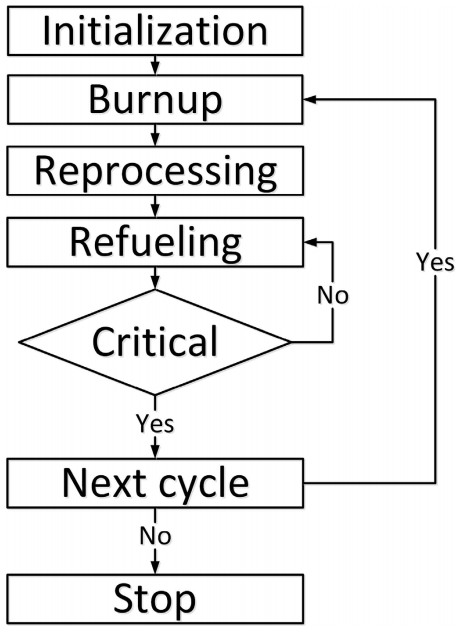
\includegraphics[height=0.4\textwidth]{./images/batch-wise.png}
	\caption{Typical flowchart for batch-wise reprocessing and refueling 
		\cite{li_optimization_2018}.}
\end{figure}               
\end{frame}


\begin{frame}
\frametitle{Fuel salt reprocessing simulation approaches pros and cons}

\begin{enumerate}
	\itemsep2em
	\item Continuous: removal and feed terms are added to the Bateman equation
	\begin{itemize}
		\itemsep1em
		\item[$\mathbf{+}$] allows coarse burnup timesteps
		\item[$\mathbf{-}$] requires a sophisticated algorithm for rebalancing 
		the salt mass 
	\end{itemize}
	\item \textbf{Batch-wise}: burnup simulation stops and restarts with 
	modified fuel composition
	\begin{itemize}
		\itemsep1em
		\item[$\mathbf{+}$] composition calculation models removals and feeds 
		at each stop/start
		\item[$\mathbf{+}$] easy to balance the salt mass in the primary loop
		\item[$\mathbf{-}$] requires very fine burnup timesteps
	\end{itemize}
\end{enumerate}
\end{frame}


\begin{frame}
\frametitle{Published work in on-line reprocessing and modeling}

  \begin{textblock*}{12.5cm}(0.1cm,1.6cm) % {block width} (coords)
	\begin{table}[t]
	\fontsize{7}{9}\selectfont
	\caption{Tools and methods for liquid-fueled \gls{MSR} fuel depletion 
	analysis.}
			\vspace{-2mm}
	\begin{tabularx}{\textwidth}{p{2.5cm} X X X p{3cm}} 
		\hline 
		&Nuttin \emph{et al.}, 2005 \cite{nuttin_potential_2005}& Aufiero \emph{et al.}, 
		2013 \cite{aufiero_extended_2013} & Betzler \emph{et al.}, 2018 
		\cite{betzler_fuel_2018}&Proposed work \\ 
		\hline
		Neutronics & \gls{MCNP} & Serpent 2 & SCALE6.2 & Serpent 2 \\
		software   & REM &           & ORIGEN-S &  \\
	               & stochastic & stochastic & deterministic & stochastic\\ [3pt]
		Geometry  & unit cell & full-core 3D & unit cell & full-core 3D\\ [3pt]
		Removal/feed  & continuous &continuous & batch-wise & batch-wise\\ [3pt]
        Separation efficiency & fixed & fixed & fixed & \textcolor{red}{function of many parameters} \\[3pt]
        Fuel reprocessing plant & ``black box'' & ``black box'' & ``black box'' & \textcolor{red}{realistic multi-component model} \\[3pt]
        Reactivity control & continuous& continuous & batch feed & 
        \textcolor{red}{periodic adjustment of geometry and fissile material 
        injection}\\[3pt]
        Power level & \multicolumn{3}{c}{fixed}& \textcolor{red}{variable} 
        \\[3pt]
		Thermal feedback & Doppler only & Not considered & Doppler only & 
		Doppler$+$\textcolor{red}{density+thermal expansion}\\[3pt]
		Void coefficient  & \multicolumn{3}{c}{Not considered} & 
		\textcolor{red}{For BOL and EOL} \\[3pt]
		Control rod worth & \multicolumn{3}{c}{Not considered} & 
		\textcolor{red}{Total} \\[3pt]
		\hline
	\end{tabularx}
	\label{tab:msr_codes}
\end{table}
\end{textblock*}

\end{frame}


\begin{frame}
\frametitle{Technical gap in the state of the art}
\vspace{-0.2in}
\begin{block}{Static ``black'' box assumptions in the literature}
	\begin{equation*}
	{\tiny  
		\setlength{\abovedisplayskip}{6pt}
		\setlength{\belowdisplayskip}{\abovedisplayskip}
		\setlength{\abovedisplayshortskip}{0pt}
		\setlength{\belowdisplayshortskip}{3pt}
	\begin{aligned}
	\begin{bmatrix}
	N^{in}_{0} \\ \vdots \\ N^{in}_{e} \\ \vdots \\ N^{in}_{E} \\
	\end{bmatrix} 
	\times
	\begin{bmatrix}
	\epsilon_{0} \\ \vdots \\ \epsilon_{e} \\ \vdots \\ \epsilon_{E} \\
	\end{bmatrix} =
	\begin{bmatrix}
	N^{out}_{0}\\ \vdots \\ N^{out}_{e} \\ \vdots \\N^{out}_{E}  \\
	\end{bmatrix}
	\end{aligned}
	}
	\end{equation*}
	\begin{itemize}
		\item \textbf{Assume time-independent separation efficiency ($\epsilon_e$).} Realistically, 
		it is \textbf{time-dependent}.
		\item \textbf{Assume $\epsilon_e$ is independent of the reactor operational 
		parameters.} But $\epsilon_e$ depends on \textbf{temperature, power level, current fuel salt isotopic composition, and material flow rate}.
		\item \textbf{Processing plant is lumped in a single ``black	box'' component.} But the system contains many components connected in series, parallel, or both. 
	\end{itemize}
\end{block}
\end{frame}

\subsection{Research objectives}

\begin{frame}
  \frametitle{Research objectives of purposed work}
                  \vspace*{-0.05in}
      The main objective of the proposed work is to develop the on-line  
      reprocessing simulation package, SaltProc, for liquid-fueled reactors 
      depletion simulations.
     \begin{block}{SaltProc desired capabilities:}<1-4>
         \begin{enumerate}
         		%\itemsep1em
                \item \textbf{Open-source} with continuous tests and 
				automatic documentation system 
                \item \textbf{Realistic} multi-component fuel 
                reprocessing system modeling
                \item Reactivity control by \textbf{changing geometry} of 
                the core during simulation
                \item \textbf{Variable} extraction efficiency support defined 
                as function of many parameters
         \end{enumerate}
      \end{block}
            \vspace{-0.1in}
	\begin{block}{SaltProc demonstration and validation for TAP MSR and 
	MSBR}<2-4>
		\begin{enumerate}
			\item<2-4> \textbf{Lifetime-long} depletion with ideal/realistic 
			$\epsilon_e$
			\item<3-4> Short-term depletion \textbf{during load-following 
			transient}
			\item<4> Safety parameters ($\alpha_{T}, \alpha_{V}$, control rod 
			worth) \textbf{evolution during long- and short-term operation}
		\end{enumerate}
	\end{block}
\end{frame}
